\usetikzlibrary{matrix}
\chapter{Algoritmo Gen\'etico}\label{chapter:ga}

En este capítulo se describe el procedimiento completo mediante el cual un algoritmo genético es utilizado para explorar estructuras posibles de modelos 
compartimentales, representadas como grafos dirigidos, que se ajusten a datos observados. El objetivo de esta búsqueda es identificar configuraciones 
estructurales que, al ser convertidas en sistemas de ecuaciones diferenciales ordinarias, permitan reproducir de manera precisa la dinámica observada en 
los datos experimentales. La naturaleza combinatoria del espacio de posibles grafos hace inviable una exploración exhaustiva, por lo que se recurre a estrategias 
evolutivas que permiten navegar dicho espacio de forma eficiente.

En la Sección~\ref{sec:init_gen} se introduce el proceso de inicialización, que establece las condiciones de partida para la ejecución del algoritmo y genera la 
población inicial de grafos candidatos. La Sección~\ref{sec:cross_gen} aborda las estrategias de recombinación empleadas para crear nuevas soluciones a partir de 
grafos existentes. En la Sección~\ref{sec:mut_gen} se explica cómo se introduce variación adicional mediante modificaciones puntuales en la estructura de los grafos. 
Finalmente, la Sección~\ref{sec:seleccion} presenta el criterio utilizado para decidir qué individuos permanecen en la población de una generación a otra y describe 
el funcionamiento general del ciclo evolutivo, que guía la búsqueda iterativa de soluciones cada vez más adecuadas.

A continuación, se describe el procedimiento de inicialización del algoritmo, donde se definen los parámetros de control y se genera la población inicial de grafos.

\section{Inicio del Algoritmo Genético}
\label{sec:init_gen}

El proceso comienza con la fase de inicialización, donde se definen los parámetros necesarios para ejecutar el algoritmo genético. Estos parámetros controlan 
el comportamiento general del algoritmo y su capacidad para explorar distintas soluciones \cite{Goldberg1989, Eiben2015}.

Primero, se establece el número de generaciones, que indica cuántos ciclos evolutivos se realizarán. Un ciclo evolutivo es el proceso completo en el que se 
generan nuevos individuos, se evalúan mediante la función \textit{fitness} y luego se seleccionan los mejores para formar la siguiente generación \cite{Goldberg1989}. 

Cada generación corresponde a una iteración del algoritmo, en la que se crean nuevos individuos, en este caso grafos, a partir de los existentes. También se define 
el tamaño de la población, que es la cantidad de grafos que existirán simultáneamente en cada generación.

Otros parámetros importantes son las tasas de cruzamiento y de mutación. La tasa de cruzamiento determina cuántos grafos nuevos se crearán combinando partes de 
grafos anteriores, mientras que la tasa de mutación establece cuántos grafos modifica aleatoriamente para introducir nuevas variantes \cite{Holland1992, Goldberg1989}. 
Estos dos mecanismos exploran el espacio de soluciones y evitar que el algoritmo se estanque en óptimos locales \cite{Holland1992, Goldberg1989}. 

Además, se inicializa una estructura que almacena todos los grafos ya evaluados. Esta estructura permite evitar la repetición de soluciones y para que el algoritmo no 
explore siempre las mismas regiones del espacio de búsqueda \cite{Eiben2015}.

Tras definir los parámetros iniciales, se genera la población inicial. Cada individuo de esta población es un grafo dirigido que representa una posible 
estructura de modelo compartimental. Estos grafos se generan aleatoriamente y se representan mediante una matriz de adyacencia, en la cual una entrada en la 
posición $(i, j)$ indica la existencia de una arista dirigida desde el nodo $i$ hacia el nodo $j$.

Sin embargo, no cualquier grafo es válido. Debe cumplir dos condiciones: no puede contener conexiones de un nodo consigo mismo y debe ser conexo cuando se interpreta 
como grafo no dirigido. Esto asegura que todos los compartimentos del modelo estén interrelacionados y que ninguna parte del sistema quede aislada. Solo los grafos 
que cumplen estas condiciones y no han sido generados previamente se incorporan a la población inicial como candidatos válidos para ser evaluados.

Después de generar la población inicial y asegurar que todos los grafos cumplan con las condiciones establecidas, el siguiente paso es aplicar los mecanismos de 
cruzamiento y mutación. Estas operaciones, que se abordarán en las siguientes secciones, permiten modificar y combinar grafos con el objetivo de explorar nuevas 
estructuras y mejorar la calidad de los modelos compartimentales generados.

\section{Proceso de Cruzamiento}
\label{sec:cross_gen}

En esta implementación, el cruzamiento se basa en la técnica clásica de un punto, ampliamente utilizada en algoritmos genéticos \cite{Goldberg1989, Eiben2015}. El 
proceso comienza con la selección aleatoria de un punto de cruce, que corresponde a una fila dentro de la matriz de adyacencia del grafo. A partir de este punto, 
se construye una nueva matriz que contiene las filas superiores de un padre y las inferiores del otro. En la Figura~\ref{fig:cruzamiento-filas} se muestra un ejemplo 
de cruzamiento por filas con punto de cruce.

\begin{figure}[htbp]
\centering

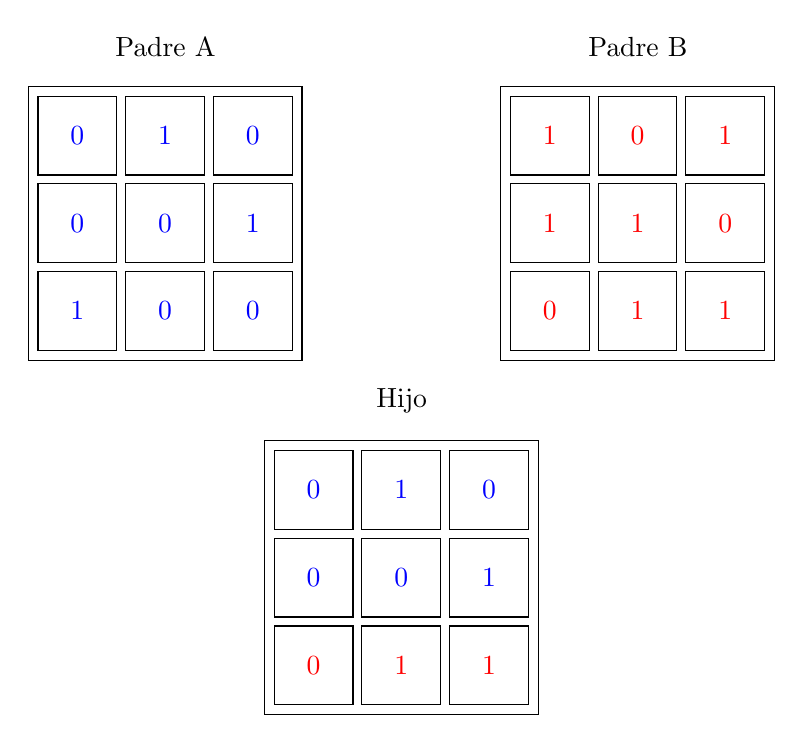
\begin{tikzpicture}
    % Padre A
\node at (1.75,0.5) {Padre A};
\matrix (A) [matrix of nodes, nodes in empty cells,
nodes={minimum size=1cm, text centered, draw},
column sep=0.1cm, row sep=0.1cm, anchor=north west,
draw=black] at (0,0)
{
    \textcolor{blue}{0} & \textcolor{blue}{1} & \textcolor{blue}{0} \\
    \textcolor{blue}{0} & \textcolor{blue}{0} & \textcolor{blue}{1} \\
    \textcolor{blue}{1} & \textcolor{blue}{0} & \textcolor{blue}{0} \\
};
    
% Padre B
\node at (7.75,0.5) {Padre B};
\matrix (B) [matrix of nodes, nodes in empty cells,
nodes={minimum size=1cm, text centered, draw},
column sep=0.1cm, row sep=0.1cm, anchor=north west,
draw=black] at (6,0)
{
    \textcolor{red}{1} & \textcolor{red}{0} & \textcolor{red}{1} \\
    \textcolor{red}{1} & \textcolor{red}{1} & \textcolor{red}{0} \\
    \textcolor{red}{0} & \textcolor{red}{1} & \textcolor{red}{1} \\
};
    
    % Hijo
\node at (4.75,-4.0) {Hijo};
\matrix (H) [matrix of nodes, nodes in empty cells,
nodes={minimum size=1cm, text centered, draw},
column sep=0.1cm, row sep=0.1cm, anchor=north west,
draw=black] at (3,-4.5)
{
    \textcolor{blue}{0} & \textcolor{blue}{1} & \textcolor{blue}{0} \\
    \textcolor{blue}{0} & \textcolor{blue}{0} & \textcolor{blue}{1} \\
    \textcolor{red}{0} & \textcolor{red}{1} & \textcolor{red}{1} \\
};

\end{tikzpicture}
\caption{Ejemplo de cruzamiento con punto de cruce en la fila 2.}
\label{fig:cruzamiento-filas}
\end{figure}

Si este hijo del cruzamiento de punto de cruce por filas cumple con los criterios de validez mencionados en secciones anteriores, se agrega como parte de la población. 
En caso contrario, se intenta un segundo tipo de cruzamiento: el cruzamiento por columnas.

En este método alternativo, se selecciona un punto de corte vertical. La parte izquierda de la matriz del hijo proviene de un padre, y la parte derecha del otro. Este 
procedimiento también requiere validación posterior. La Figura~\ref{fig:cruzamiento-columnas} ilustra este segundo tipo de cruzamiento. Si tampoco cumple las 
condiciones de validez, el intento de cruzamiento se descarta y no se añade ningún nuevo individuo a la población desde esa pareja de padres.

\begin{figure}[htbp]
\centering
    
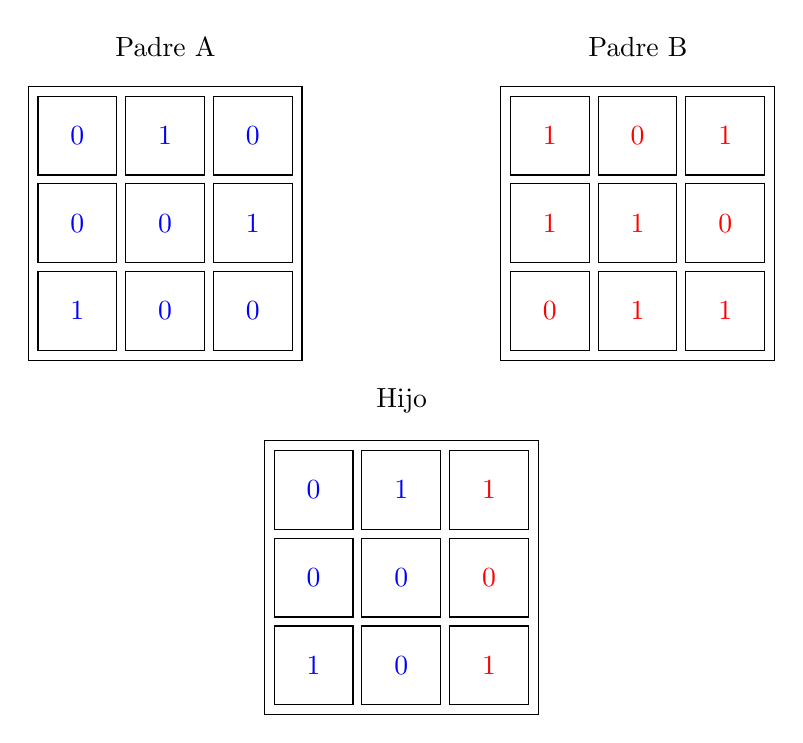
\begin{tikzpicture}
        % Padre A
\node at (1.75,0.5) {Padre A};
\matrix (A) [matrix of nodes, nodes in empty cells,
nodes={minimum size=1cm, text centered, draw},
column sep=0.1cm, row sep=0.1cm, anchor=north west,
draw=black] at (0,0)
{
    \textcolor{blue}{0} & \textcolor{blue}{1} & \textcolor{blue}{0} \\
    \textcolor{blue}{0} & \textcolor{blue}{0} & \textcolor{blue}{1} \\
    \textcolor{blue}{1} & \textcolor{blue}{0} & \textcolor{blue}{0} \\
};
        
    % Padre B
\node at (7.75,0.5) {Padre B};
\matrix (B) [matrix of nodes, nodes in empty cells,
nodes={minimum size=1cm, text centered, draw},
column sep=0.1cm, row sep=0.1cm, anchor=north west,
draw=black] at (6,0)
{
    \textcolor{red}{1} & \textcolor{red}{0} & \textcolor{red}{1} \\
    \textcolor{red}{1} & \textcolor{red}{1} & \textcolor{red}{0} \\
    \textcolor{red}{0} & \textcolor{red}{1} & \textcolor{red}{1} \\
};
        
        % Hijo
\node at (4.75,-4.0) {Hijo};
\matrix (H) [matrix of nodes, nodes in empty cells,
nodes={minimum size=1cm, text centered, draw},
column sep=0.1cm, row sep=0.1cm, anchor=north west,
draw=black] at (3,-4.5)
{
    \textcolor{blue}{0} & \textcolor{blue}{1} & \textcolor{red}{1} \\
    \textcolor{blue}{0} & \textcolor{blue}{0} & \textcolor{red}{0} \\
    \textcolor{blue}{1} & \textcolor{blue}{0} & \textcolor{red}{1} \\
};
    
\end{tikzpicture}
\caption{Ejemplo de cruzamiento con punto de cruce en la columna 2.}
\label{fig:cruzamiento-columnas}
\end{figure}

Al aplicar distintos métodos de recombinación, el algoritmo aumenta sus posibilidades de generar soluciones viables que podrían no surgir con un único tipo de 
cruzamiento \cite{Eiben2015}.

Una vez generados nuevos grafos mediante cruzamiento, estos se evalúan en la función \textit{fitness} y se incorporan a la población como posibles soluciones 
para la siguiente generación, lo cual es un paso estándar en el ciclo de los algoritmos genéticos \cite{Eiben2015}. A continuación, se describe el proceso de 
mutación y su papel en la diversidad genética del algoritmo.

\section{Proceso de Mutación}
\label{sec:mut_gen}

En el caso de que los individuos sean grafos dirigidos, existen tres tipos principales de mutaciones que se pueden aplicar directamente sobre su matriz de adyacencia:

\begin{itemize}
    \item \textbf{Eliminación de una arista}: se selecciona aleatoriamente una posición $(i,j)$ de la matriz que contiene un 1 
    (indicando una arista de \(X_i \rightarrow X_j\)) y se cambia a 0. Esta operación solo se ejecuta si no rompe la conexidad del grafo cuando se interpreta como no 
    dirigido.
    
    \item \textbf{Adición de una arista}: se escoge aleatoriamente una celda $(i,j)$ de la matriz de adyacencia que contenga un 0 y se cambia a 1, creando una nueva 
    arista dirigida \(X_i \rightarrow X_j\), siempre que esta conexión no exista previamente.

    \item \textbf{Cambio de dirección de una arista}: se elige una arista existente $(i,j)$, se elimina (poniendo un 0 en esa posición) y se añade la arista inversa 
    $(j,i)$ (poniendo un 1), siempre que esta última no esté ya presente.
\end{itemize}

La Figura~\ref{fig:mutaciones-ejemplo} ilustra estos tres tipos de mutación mediante operaciones sobre matrices de adyacencia.


\begin{figure}[htbp]
\centering
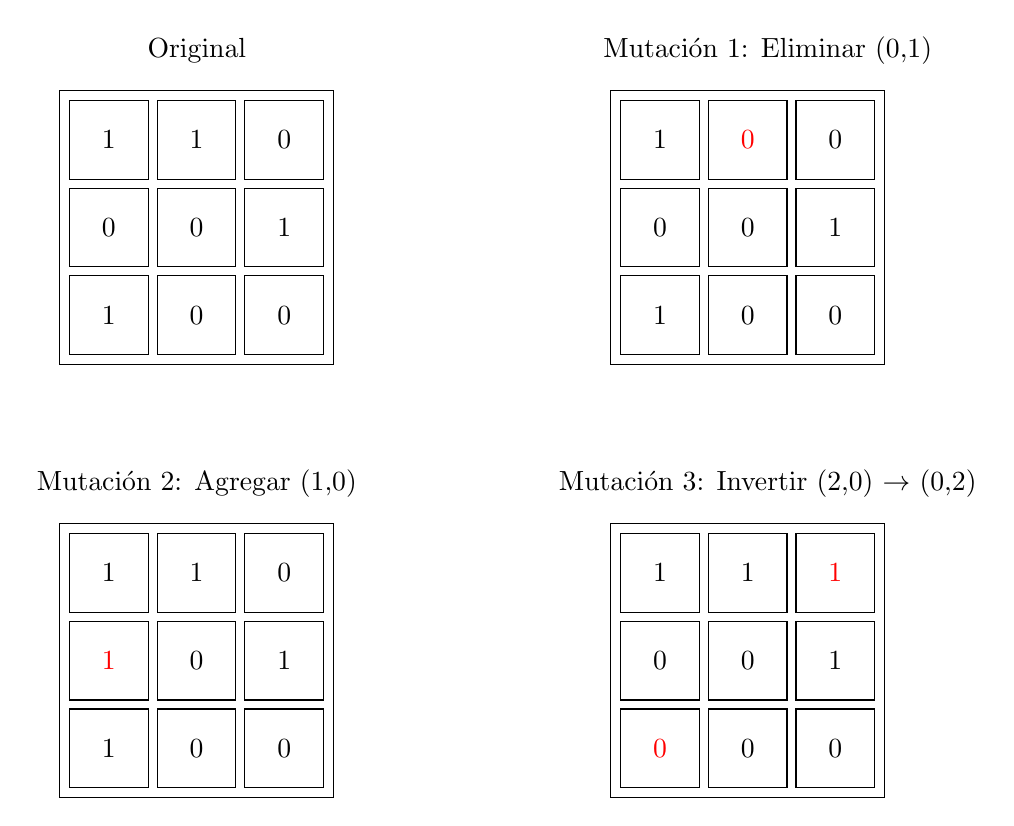
\begin{tikzpicture}
    
    % Original
\node at (1.75,1.5) {Original};
\matrix (O) [matrix of nodes, nodes in empty cells,
nodes={minimum size=1cm, text centered, draw},
column sep=0.1cm, row sep=0.1cm, anchor=north west,
draw=black] at (0,1)
{
    \textcolor{black}{1} & \textcolor{black}{1} & \textcolor{black}{0} \\
    \textcolor{black}{0} & \textcolor{black}{0} & \textcolor{black}{1} \\
    \textcolor{black}{1} & \textcolor{black}{0} & \textcolor{black}{0} \\
};
    
    % Mutación 1 - Eliminar arista (0,1)
\node at (9,1.5) {Mutación 1: Eliminar (0,1)};
\matrix (M1) [matrix of nodes, nodes in empty cells,
nodes={minimum size=1cm, text centered, draw},
column sep=0.1cm, row sep=0.1cm, anchor=north west,
draw=black] at (7,1)
{
    \textcolor{black}{1} & \textcolor{red}{0} & \textcolor{black}{0} \\
    \textcolor{black}{0} & \textcolor{black}{0} & \textcolor{black}{1} \\
    \textcolor{black}{1} & \textcolor{black}{0} & \textcolor{black}{0} \\
};
    
    % Mutación 2 - Agregar arista (1,0)
\node at (1.75,-4.0) {Mutación 2: Agregar (1,0)};
\matrix (M2) [matrix of nodes, nodes in empty cells,
nodes={minimum size=1cm, text centered, draw},
column sep=0.1cm, row sep=0.1cm, anchor=north west,
draw=black] at (0,-4.5)
{
    \textcolor{black}{1} & \textcolor{black}{1} & \textcolor{black}{0} \\
    \textcolor{red}{1} & \textcolor{black}{0} & \textcolor{black}{1} \\
    \textcolor{black}{1} & \textcolor{black}{0} & \textcolor{black}{0} \\
};
    
% Mutación 3 - Invertir dirección (2,0) -> (0,2)
\node at (9,-4.0) {Mutación 3: Invertir (2,0) $\rightarrow$ (0,2)};
\matrix (M3) [matrix of nodes, nodes in empty cells,
nodes={minimum size=1cm, text centered, draw},
column sep=0.1cm, row sep=0.1cm, anchor=north west,
draw=black] at (7,-4.5)
{
    \textcolor{black}{1} & \textcolor{black}{1} & \textcolor{red}{1} \\
    \textcolor{black}{0} & \textcolor{black}{0} & \textcolor{black}{1} \\
    \textcolor{red}{0} & \textcolor{black}{0} & \textcolor{black}{0} \\
};
    
\end{tikzpicture}
\caption{Ejemplos de mutaciones: eliminación, adición e inversión de aristas.}
\label{fig:mutaciones-ejemplo}
\end{figure}


En todos los casos, el grafo resultante debe cumplir con las restricciones estructurales del problema: debe permanecer conexo cuando se considera no dirigido y no debe 
haberse evaluado anteriormente. Para verificar que los grafos no han sido procesados se realiza una consulta en una tabla hash que almacena representaciones canónicas 
de los grafos ya analizados, y para comprobar la conexidad del sistema compartimental dado que los grafos en este contexto son dirigidos, la verificación de su 
conectividad se realiza sobre una versión no dirigida. Para ello, se construye una matriz simétrica \(A^{\text{undir}}\) combinando la matriz de adyacencia original 
\(A\) con su transpuesta mediante \(A^{\text{undir}}_{ij} = A_{ij} \lor A_{ji}\). Esta matriz representa un grafo no dirigido en el que se considera que hay conexión 
entre dos nodos si existe una arista en al menos una dirección. Usando la biblioteca \texttt{networkx} \cite{Hagberg2008}, se crea el grafo correspondiente y se aplica el método 
\texttt{is\_connected()} para comprobar que todos los nodos pertenecen al mismo componente conexo.

Si una mutación genera una estructura inválida ,por ejemplo un grafo evaluado anteriormente, el algoritmo descarta ese hijo y no lo agrega
a la población.

Una vez que se han generado nuevos grafos mediante cruzamiento y mutación, es necesario evaluar su calidad y decidir cuáles de ellos pasarán a la siguiente generación. 
No todos los individuos producidos en una iteración deben conservarse, por lo que se aplica un proceso de selección que permite retener aquellos grafos que mejor se 
ajustan a los datos. Esta etapa es clave para garantizar que el algoritmo evolucione hacia soluciones o\'ptimas lo que se aborda en la siguiente sección.

\section{Selección y evolución del algoritmo}
\label{sec:seleccion}

Después de aplicar las operaciones de cruzamiento y mutación, los nuevos grafos generados deben ser evaluados para determinar su capacidad de ajustarse a los datos. 
Esta evaluación se realiza con la función \textit{fitness}.

Solo se analizan los grafos que aún no han sido evaluados previamente, evitando así repeticiones innecesarias que no aportarían nueva información.

Los grafos nuevos se a\~naden a los de la generación anterior para formar una población ampliada. Esta población ampliada representa el conjunto completo de 
candidatos disponibles para la selección en la siguiente etapa. A esta población ampliada se le aplica un proceso de ordenamiento según el valor de \textit{fitness}, 
seleccionando los mejores $N$ individuos, donde $N$ es el tamaño original de la población inicial, para conformar la nueva generación. Este enfoque, conocido como 
selección elitista, garantiza que las soluciones prometedoras se conserven, mientras se incorporan también estructuras nuevas que pueden mejorar los resultados 
\cite{Eiben2015, Goldberg1989}.

Al finalizar todas las generaciones, el algoritmo retorna un conjunto de grafos con los mejores desempeños según la métrica de \textit{fitness}. Cada grafo describe 
cómo se conectan e interactúan los distintos compartimentos del modelo, determinando qué flujos de información o cantidad existen entre ellos.

En este capítulo se presentó el funcionamiento completo del algoritmo genético diseñado para explorar el espacio de modelos compartimentales representados por grafos 
dirigidos. Se detallaron los mecanismos que guían la evolución de la población de soluciones, incluyendo la generación inicial de grafos válidos, las operaciones de 
cruzamiento y mutación para introducir variabilidad estructural, y el proceso de selección que preserva los candidatos más prometedores. A lo largo del ciclo evolutivo, 
el algoritmo garantiza la validez topológica de los grafos, evita la repetición de individuos previamente evaluados y se orienta hacia configuraciones que maximizan la 
función de \textit{fitness}. Este enfoque evolutivo permite una búsqueda eficiente y estructurada de modelos dinámicos, manteniendo un equilibrio entre 
exploración del espacio de soluciones y explotación de los mejores resultados encontrados.

En el siguiente capítulo se presentan los experimentos y resultados obtenidos al aplicar la implementación propuesta a diferentes modelos compartimentales.